\documentclass[border=5pt]{standalone}
\usepackage{fontspec}
\usepackage{unicode-math}
\setmainfont{Noto Serif}
\newfontfamily\FigureItalic{Noto Serif}
\setmathfont{STIXTwoMath-Regular.otf}
\usepackage{tikz}
\usetikzlibrary{arrows.meta,calc,patterns,decorations.pathmorphing,decorations.markings,decorations.pathreplacing,positioning,backgrounds}
\definecolor{Ink}{HTML}{000000}
\definecolor{Curve}{HTML}{000000}
\definecolor{Bzero}{HTML}{000000}
\definecolor{Bone}{HTML}{000000}
\definecolor{Btwo}{HTML}{000000}
\definecolor{Bthree}{HTML}{000000}
\definecolor{Bfour}{HTML}{000000}
\tikzset{
 ax/.style={draw=Ink,line width=.72pt,-{Latex[length=2.4mm,width=1.5mm]}},
 lev/.style={draw=Ink,line width=1.4pt,line cap=butt},
 thinlev/.style={draw=Ink,line width=.65pt,line cap=butt},
 helper/.style={draw=Ink,line width=.65pt},
 bare/.style={draw=Ink,line width=.95pt,dash pattern=on 4pt off 2.8pt},
 curve/.style={draw=Ink,line width=1.85pt,line cap=round,line join=round},
 ray/.style={draw=Ink,line width=1.0pt,-{Latex[length=2.3mm,width=1.4mm]}},
 measure/.style={draw=Ink,line width=.75pt,{Latex[length=1.9mm,width=1.2mm]}-{Latex[length=1.9mm,width=1.2mm]}},
 link/.style={draw=Ink,line width=1.0pt},
 wave/.style={draw=Ink,line width=.85pt,decorate,decoration={snake,amplitude=.33mm,segment length=2.5mm,pre length=.8mm,post length=.8mm}},
 photon/.style={draw=Ink,line width=1.0pt,-{Latex[length=2.0mm,width=1.3mm]},decorate,decoration={snake,amplitude=.4mm,segment length=2.7mm,pre length=0mm,post length=1.9mm}},
 lab/.style={text=Ink,font=\fontsize{13.5}{16}\selectfont,inner sep=2pt},
 small/.style={text=Ink,font=\fontsize{11.5}{14}\selectfont,inner sep=2pt},
 tag/.style={text=Ink,font=\fontsize{14}{17}\selectfont\FigureItalic\itshape,inner sep=2pt}}
\pagestyle{empty}

\begin{document}
% Figure 13.8; source-grounded revision.
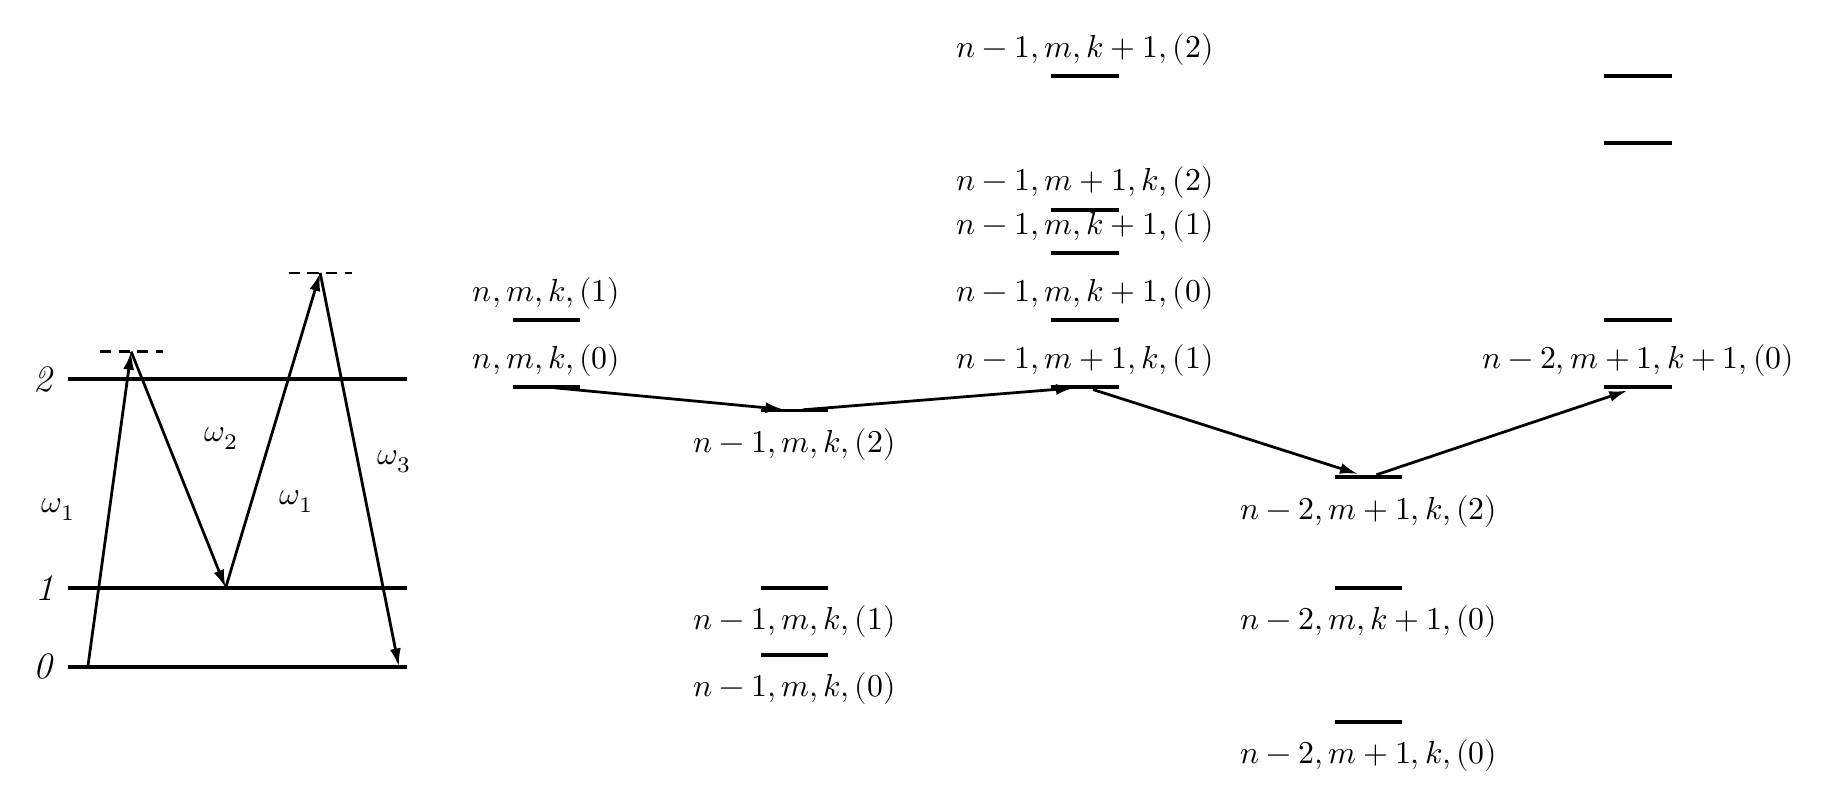
\begin{tikzpicture}[x=1cm,y=1cm]
\coordinate (aa0) at (2.15000,0.00000);
\coordinate (aa0L) at (0.00000,0.00000);
\coordinate (aa0R) at (4.30000,0.00000);
\draw[lev] (aa0L) -- (aa0R);
\node[lab,anchor=east] at (-0.10000,0.00000) {\textit{0}};
\coordinate (aa1) at (2.15000,1.00000);
\coordinate (aa1L) at (0.00000,1.00000);
\coordinate (aa1R) at (4.30000,1.00000);
\draw[lev] (aa1L) -- (aa1R);
\node[lab,anchor=east] at (-0.10000,1.00000) {\textit{1}};
\coordinate (aa2) at (2.15000,3.65000);
\coordinate (aa2L) at (0.00000,3.65000);
\coordinate (aa2R) at (4.30000,3.65000);
\draw[lev] (aa2L) -- (aa2R);
\node[lab,anchor=east] at (-0.10000,3.65000) {\textit{2}};
\coordinate (v1) at (0.80000,4.00000);
\draw[bare] (0.40000,4.00000) -- (1.20000,4.00000);
\coordinate (v2) at (3.20000,5.00000);
\draw[bare] (2.80000,5.00000) -- (3.60000,5.00000);
\draw[ray] (0.25000,0.00000) -- (v1);
\draw[ray] (v1) -- (2.00000,1.00000);
\draw[ray] (2.00000,1.00000) -- (v2);
\draw[ray] (v2) -- (4.20000,0.00000);
\node[small] at (-0.12000,2.00000) {$\omega_1$};
\node[small] at (1.95000,2.90000) {$\omega_2$};
\node[small] at (2.90000,2.10000) {$\omega_1$};
\node[small] at (4.15000,2.60000) {$\omega_3$};
\node[tag] at (1.80000,-0.65000) {а};
\begin{scope}[xscale=.90,xshift=.65cm]
\coordinate (g0_0) at (6.10000,4.40000);
\coordinate (g0_0L) at (5.62500,4.40000);
\coordinate (g0_0R) at (6.57500,4.40000);
\draw[lev] (g0_0L) -- (g0_0R);
\node[small] at (6.10000,4.74000) {$n,m,k,(1)$};
\coordinate (g0_1) at (6.10000,3.55000);
\coordinate (g0_1L) at (5.62500,3.55000);
\coordinate (g0_1R) at (6.57500,3.55000);
\draw[lev] (g0_1L) -- (g0_1R);
\node[small] at (6.10000,3.89000) {$n,m,k,(0)$};
\coordinate (g1_0) at (9.60000,3.25250);
\coordinate (g1_0L) at (9.12500,3.25250);
\coordinate (g1_0R) at (10.07500,3.25250);
\draw[lev] (g1_0L) -- (g1_0R);
\node[small] at (9.60000,2.82250) {$n-1,m,k,(2)$};
\coordinate (g1_1) at (9.60000,1.00000);
\coordinate (g1_1L) at (9.12500,1.00000);
\coordinate (g1_1R) at (10.07500,1.00000);
\draw[lev] (g1_1L) -- (g1_1R);
\node[small] at (9.60000,0.57000) {$n-1,m,k,(1)$};
\coordinate (g1_2) at (9.60000,0.15000);
\coordinate (g1_2L) at (9.12500,0.15000);
\coordinate (g1_2R) at (10.07500,0.15000);
\draw[lev] (g1_2L) -- (g1_2R);
\node[small] at (9.60000,-0.28000) {$n-1,m,k,(0)$};
\coordinate (g2_0) at (13.70000,7.50250);
\coordinate (g2_0L) at (13.22500,7.50250);
\coordinate (g2_0R) at (14.17500,7.50250);
\draw[lev] (g2_0L) -- (g2_0R);
\node[small] at (13.70000,7.84250) {$n-1,m,k+1,(2)$};
\coordinate (g2_1) at (13.70000,5.80250);
\coordinate (g2_1L) at (13.22500,5.80250);
\coordinate (g2_1R) at (14.17500,5.80250);
\draw[lev] (g2_1L) -- (g2_1R);
\node[small] at (13.70000,6.14250) {$n-1,m+1,k,(2)$};
\coordinate (g2_2) at (13.70000,5.25000);
\coordinate (g2_2L) at (13.22500,5.25000);
\coordinate (g2_2R) at (14.17500,5.25000);
\draw[lev] (g2_2L) -- (g2_2R);
\node[small] at (13.70000,5.59000) {$n-1,m,k+1,(1)$};
\coordinate (g2_3) at (13.70000,4.40000);
\coordinate (g2_3L) at (13.22500,4.40000);
\coordinate (g2_3R) at (14.17500,4.40000);
\draw[lev] (g2_3L) -- (g2_3R);
\node[small] at (13.70000,4.74000) {$n-1,m,k+1,(0)$};
\coordinate (g2_4) at (13.70000,3.55000);
\coordinate (g2_4L) at (13.22500,3.55000);
\coordinate (g2_4R) at (14.17500,3.55000);
\draw[lev] (g2_4L) -- (g2_4R);
\node[small] at (13.70000,3.89000) {$n-1,m+1,k,(1)$};
\coordinate (g3_0) at (17.70000,2.40250);
\coordinate (g3_0L) at (17.22500,2.40250);
\coordinate (g3_0R) at (18.17500,2.40250);
\draw[lev] (g3_0L) -- (g3_0R);
\node[small] at (17.70000,1.97250) {$n-2,m+1,k,(2)$};
\coordinate (g3_1) at (17.70000,1.00000);
\coordinate (g3_1L) at (17.22500,1.00000);
\coordinate (g3_1R) at (18.17500,1.00000);
\draw[lev] (g3_1L) -- (g3_1R);
\node[small] at (17.70000,0.57000) {$n-2,m,k+1,(0)$};
\coordinate (g3_2) at (17.70000,-0.70000);
\coordinate (g3_2L) at (17.22500,-0.70000);
\coordinate (g3_2R) at (18.17500,-0.70000);
\draw[lev] (g3_2L) -- (g3_2R);
\node[small] at (17.70000,-1.13000) {$n-2,m+1,k,(0)$};
\coordinate (g4_0) at (21.50000,3.55000);
\coordinate (g4_0L) at (21.02500,3.55000);
\coordinate (g4_0R) at (21.97500,3.55000);
\draw[lev] (g4_0L) -- (g4_0R);
\node[small] at (21.50000,3.89000) {$n-2,m+1,k+1,(0)$};
\coordinate (continuation0) at (21.50000,4.40000);
\coordinate (continuation0L) at (21.02500,4.40000);
\coordinate (continuation0R) at (21.97500,4.40000);
\draw[lev] (continuation0L) -- (continuation0R);
\coordinate (continuation1) at (21.50000,6.65250);
\coordinate (continuation1L) at (21.02500,6.65250);
\coordinate (continuation1R) at (21.97500,6.65250);
\draw[lev] (continuation1L) -- (continuation1R);
\coordinate (continuation2) at (21.50000,7.50250);
\coordinate (continuation2L) at (21.02500,7.50250);
\coordinate (continuation2R) at (21.97500,7.50250);
\draw[lev] (continuation2L) -- (continuation2R);
\draw[ray,shorten <=3pt,shorten >=4pt] (g0_1) -- (g1_0);
\draw[ray,shorten <=3pt,shorten >=4pt] (g1_0) -- (g2_4);
\draw[ray,shorten <=3pt,shorten >=4pt] (g2_4) -- (g3_0);
\draw[ray,shorten <=3pt,shorten >=4pt] (g3_0) -- (g4_0);
\node[tag] at (13.80000,-1.40000) {б};
\end{scope}\end{tikzpicture}

\end{document}
